% !TeX root = ../main.tex
% Add the above to each chapter to make compiling the PDF easier in some editors.

%\chapter{PASCAL VOC Void Pixel}


\begin{figure}
	\centering
	% Bag
	\begin{subfigure}[t]{0.3\textwidth}
		\centering
		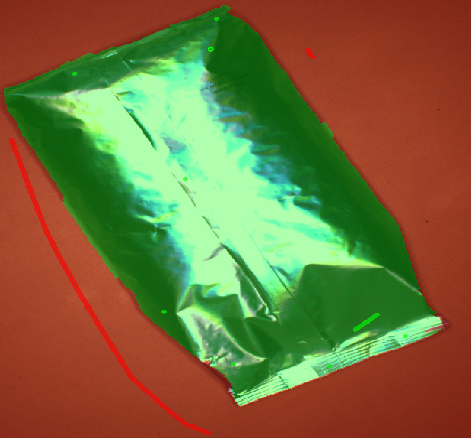
\includegraphics[width=\textwidth]{figures/appendix/method_predictions/bag21_watershed.png}
		\caption{Watershed $ IoU = 0.9799 $}
	\end{subfigure}
	\hfill
	\begin{subfigure}[t]{0.3\textwidth}
		\centering
		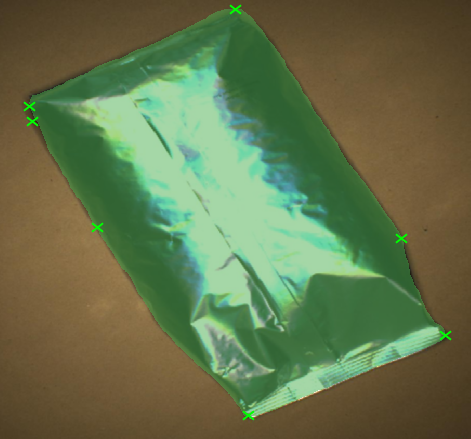
\includegraphics[width=\textwidth]{figures/appendix/method_predictions/bag21_dextr.png}
		\caption{DEXTR $ IoU = 0.9784 $}
	\end{subfigure}
	\hfill
	\begin{subfigure}[t]{0.3\textwidth}
		\centering
		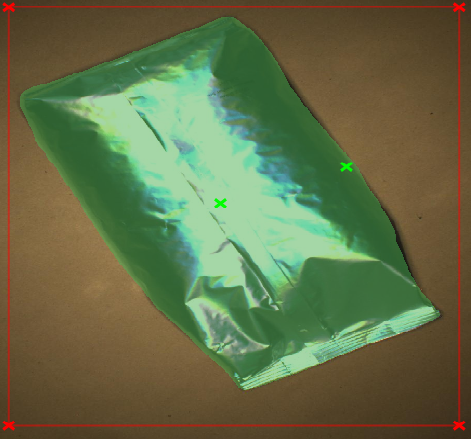
\includegraphics[width=\textwidth]{figures/appendix/method_predictions/bag21_iog.png}
		\caption{IOG $ IoU = 0.9702 $}
	\end{subfigure}
	\\
	% Cereal
	\begin{subfigure}[t]{0.3\textwidth}
		\centering
		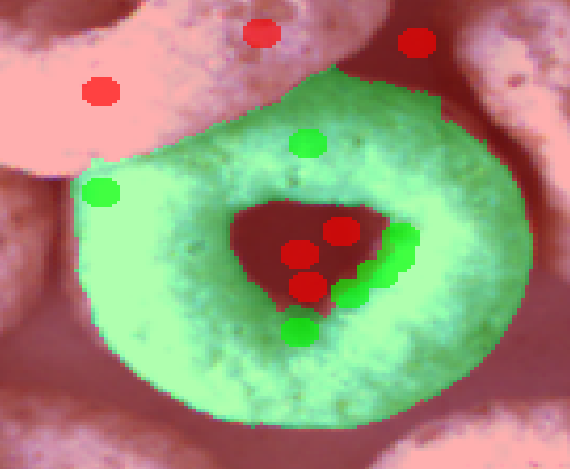
\includegraphics[width=\textwidth]{figures/appendix/method_predictions/cereal67_watershed.png}
		\caption{Watershed $ IoU = 0.9411 $}
	\end{subfigure}
	\hfill
	\begin{subfigure}[t]{0.3\textwidth}
		\centering
		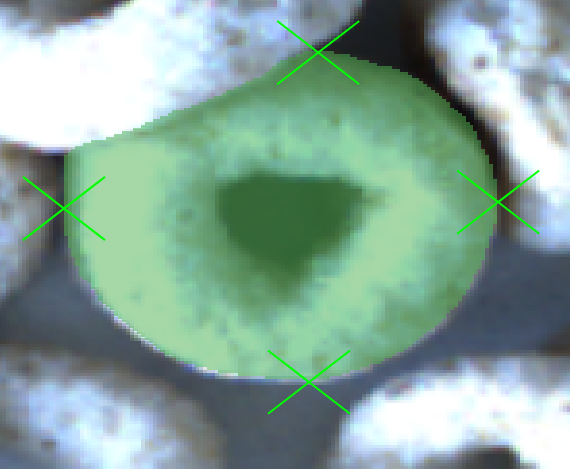
\includegraphics[width=\textwidth]{figures/appendix/method_predictions/cereal67_dextr.png}
		\caption{DEXTR $ IoU = 0.8362 $}
	\end{subfigure}
	\hfill
	\begin{subfigure}[t]{0.3\textwidth}
		\centering
		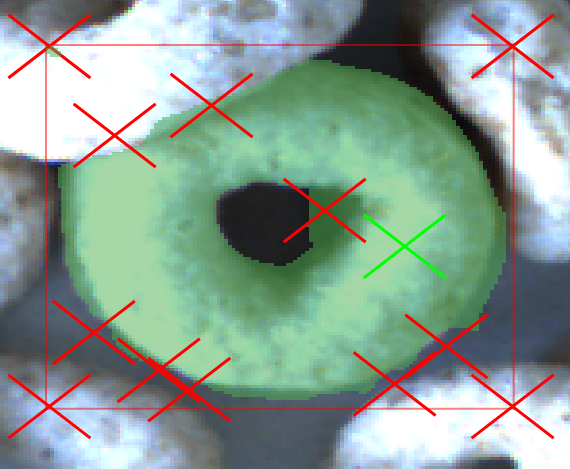
\includegraphics[width=\textwidth]{figures/appendix/method_predictions/cereal67_iog.png}
		\caption{
			IOG $ IoU = 0.8634 $
		}
	\end{subfigure}
	\\	
	% Jet
	\begin{subfigure}[t]{0.3\textwidth}
		\centering
		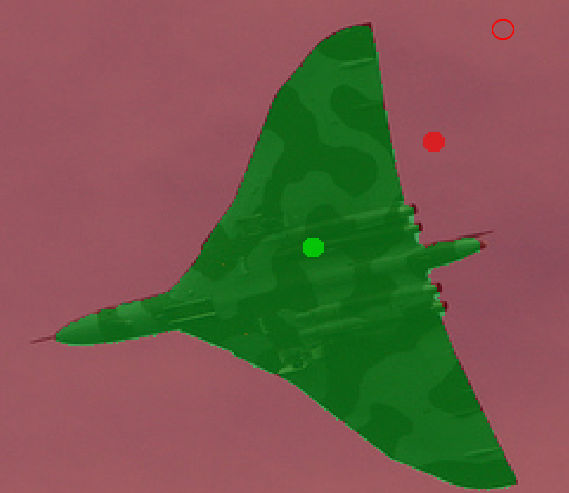
\includegraphics[width=\textwidth]{figures/appendix/method_predictions/jet4_watershed.png}
		\caption{
			Watershed $ IoU = 0.9593 $
		}
	\end{subfigure}
	\hfill
	\begin{subfigure}[t]{0.3\textwidth}
		\centering
		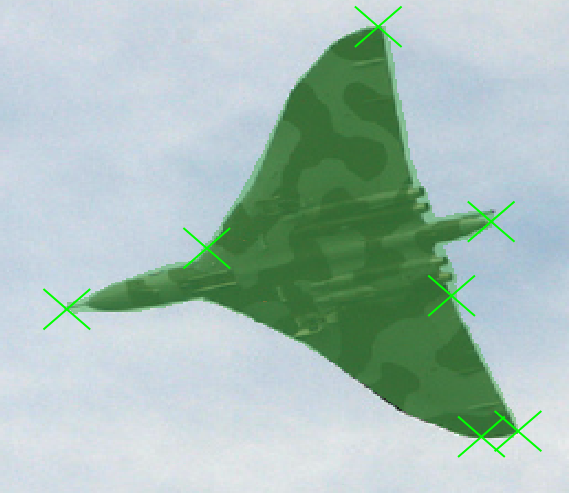
\includegraphics[width=\textwidth]{figures/appendix/method_predictions/jet4_dextr.png}
		\caption{
			DEXTR $ IoU = 0.9528 $
		}
	\end{subfigure}
	\hfill
	\begin{subfigure}[t]{0.3\textwidth}
		\centering
		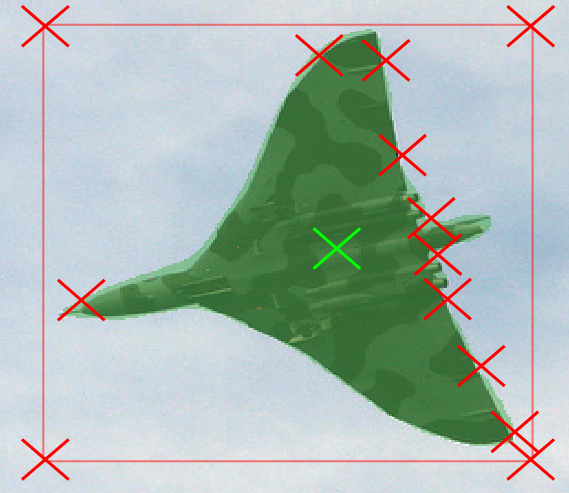
\includegraphics[width=\textwidth]{figures/appendix/method_predictions/jet4_iog.png}
		\caption{
			IOG $ IoU = 0.9429 $
		}
	\end{subfigure}
	\\	
	% Can
	\begin{subfigure}[t]{0.3\textwidth}
		\centering
		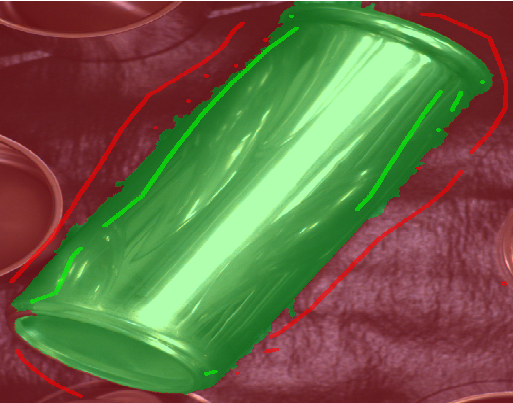
\includegraphics[width=\textwidth]{figures/appendix/method_predictions/cans75_watershed.png}
		\caption{
			Watershed $ IoU = 0.9577 $
		}
	\end{subfigure}
	\hfill
	\begin{subfigure}[t]{0.3\textwidth}
		\centering
		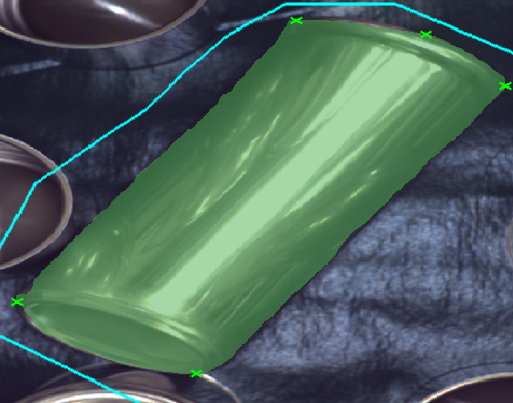
\includegraphics[width=\textwidth]{figures/appendix/method_predictions/cans75_dextr.png}
		\caption{
			DEXTR $ IoU = 0.9516 $
		}
	\end{subfigure}
	\hfill
	\begin{subfigure}[t]{0.3\textwidth}
		\centering
		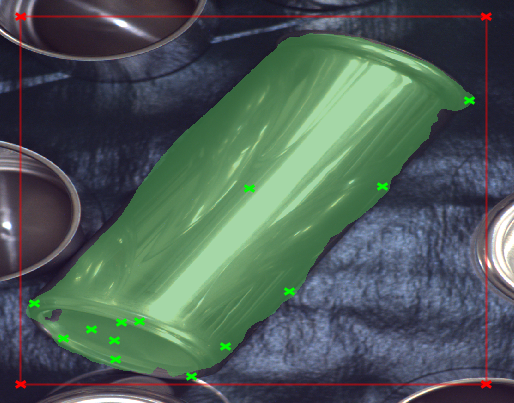
\includegraphics[width=\textwidth]{figures/appendix/method_predictions/cans75_iog.png}
		\caption{
			IOG $ IoU = 0.9289 $
		}
	\end{subfigure}
	\caption[Predictions from watershed, DEXTR, and IOG]{
		Illustration of some predictions from the methods watershed (left column), \gls{dextr} (middle column), and \gls{iog} (right column).
		The resulting $ IoU $ is presented for each prediction and in the image it can be seen how much clicks or strokes were set.
		It was aimed to create a satisfactory result, therefore, the amount of clicks and strokes differ between the methods. 
	}\label{fig:appendix_model_predictions}
\end{figure}
	
	
\begin{figure} \ContinuedFloat
	% Pill
	\begin{subfigure}[t]{0.3\textwidth}
		\centering
		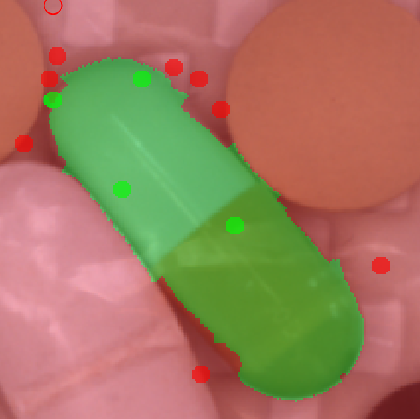
\includegraphics[width=\textwidth]{figures/appendix/method_predictions/pill56_watershed.png}
		\caption{
			Watershed $ IoU = 0.9275 $
		}
	\end{subfigure}
	\hfill
	\begin{subfigure}[t]{0.3\textwidth}
		\centering
		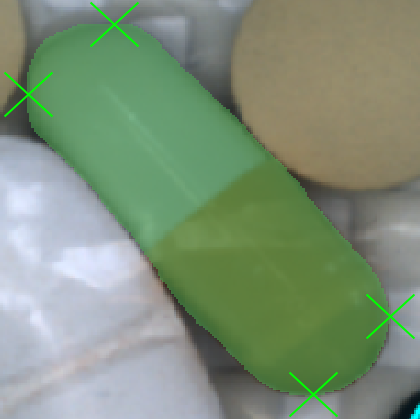
\includegraphics[width=\textwidth]{figures/appendix/method_predictions/pill56_dextr.png}
		\caption{
			DEXTR $ IoU = 0.9705 $
		}
	\end{subfigure}
	\hfill
	\begin{subfigure}[t]{0.3\textwidth}
		\centering
		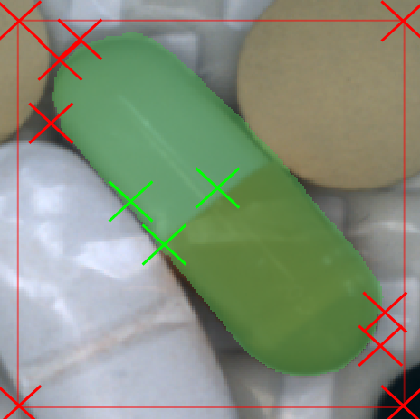
\includegraphics[width=\textwidth]{figures/appendix/method_predictions/pill56_iog.png}
		\caption{
			IOG $ IoU = 0.9482 $
		}
	\end{subfigure}
	\\	
	% Screw
	\begin{subfigure}[t]{0.3\textwidth}
		\centering
		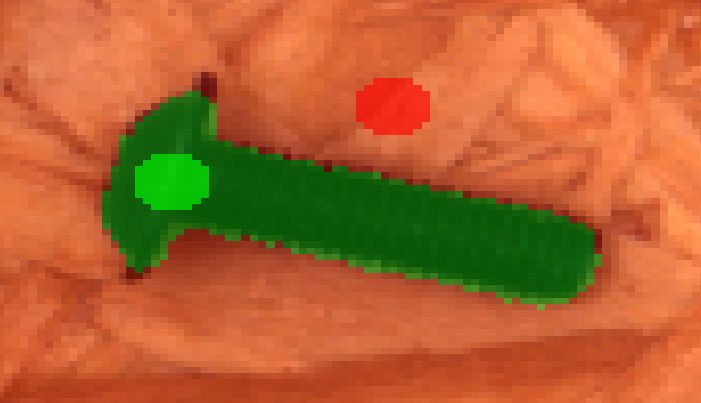
\includegraphics[width=\textwidth]{figures/appendix/method_predictions/screw57_watershed.png}
		\caption{
			Watershed $ IoU = 0.8420 $
		}
	\end{subfigure}
	\hfill
	\begin{subfigure}[t]{0.3\textwidth}
		\centering
		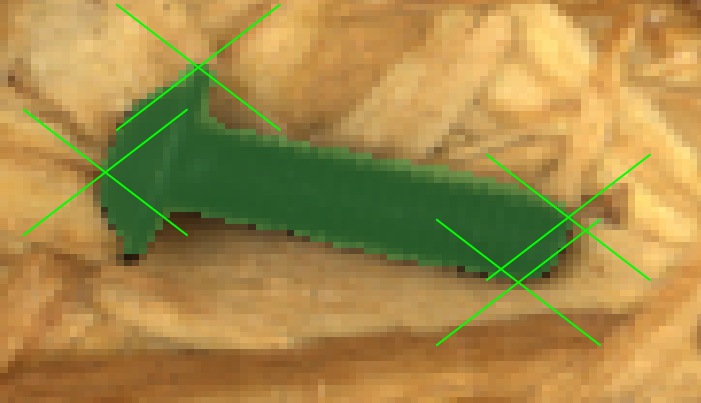
\includegraphics[width=\textwidth]{figures/appendix/method_predictions/screw57_dextr.png}
		\caption{
			DEXTR $ IoU = 0.8854 $
		}
	\end{subfigure}
	\hfill
	\begin{subfigure}[t]{0.3\textwidth}
		\centering
		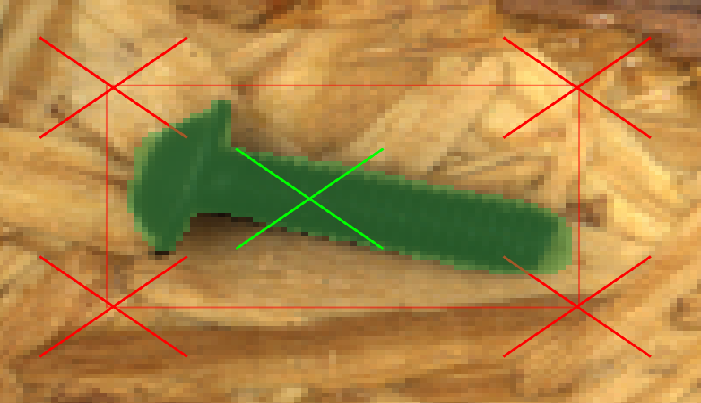
\includegraphics[width=\textwidth]{figures/appendix/method_predictions/screw57_iog.png}
		\caption{
			IOG $ IoU = 0.8734 $
		}
	\end{subfigure}
	\\
	% Tea
	\begin{subfigure}[t]{0.3\textwidth}
		\centering
		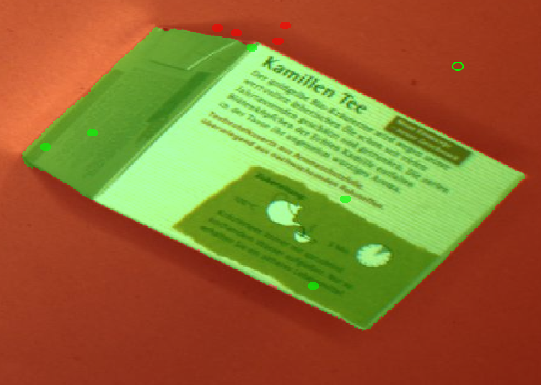
\includegraphics[width=\textwidth]{figures/appendix/method_predictions/tea17_watershed.png}
		\caption{
			Watershed $ IoU = 0.9842 $
		}
	\end{subfigure}
	\hfill
	\begin{subfigure}[t]{0.3\textwidth}
		\centering
		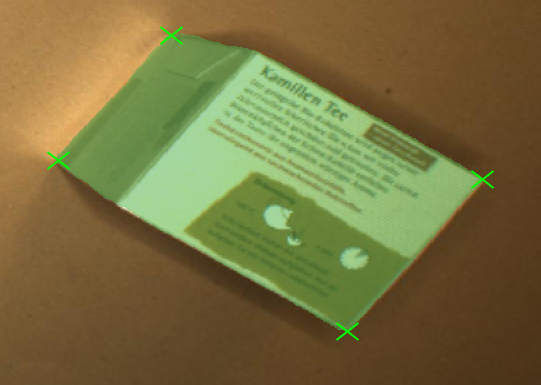
\includegraphics[width=\textwidth]{figures/appendix/method_predictions/tea17_dextr.png}
		\caption{
			DEXTR $ IoU = 0.9814 $
		}
	\end{subfigure}
	\hfill
	\begin{subfigure}[t]{0.3\textwidth}
		\centering
		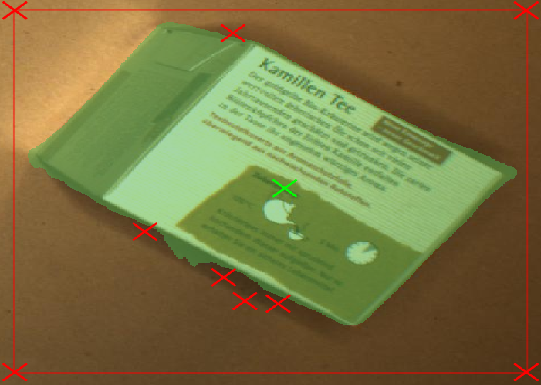
\includegraphics[width=\textwidth]{figures/appendix/method_predictions/tea17_iog.png}
		\caption{
			IOG $ IoU = 0.9438 $
		}
	\end{subfigure}
	\\
	% Swan
	\begin{subfigure}[t]{0.3\textwidth}
		\centering
		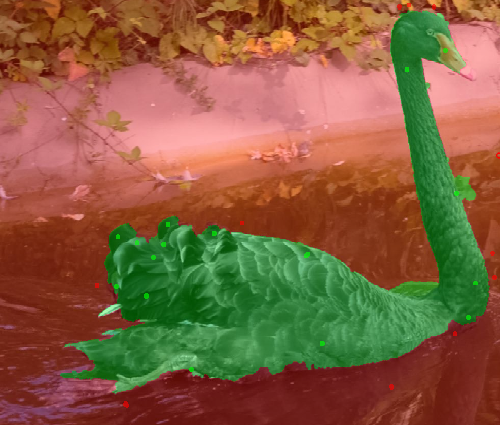
\includegraphics[width=\textwidth]{figures/appendix/method_predictions/swan34_watershed.png}
		\caption{
			Watershed $ IoU = 0.9099 $
		}
	\end{subfigure}
	\hfill
	\begin{subfigure}[t]{0.3\textwidth}
		\centering
		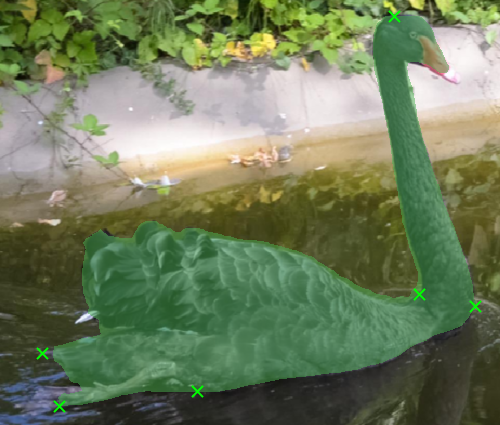
\includegraphics[width=\textwidth]{figures/appendix/method_predictions/swan34_dextr.png}
		\caption{
			DEXTR $ IoU = 0.9048 $
		}
	\end{subfigure}
	\hfill
	\begin{subfigure}[t]{0.3\textwidth}
		\centering
		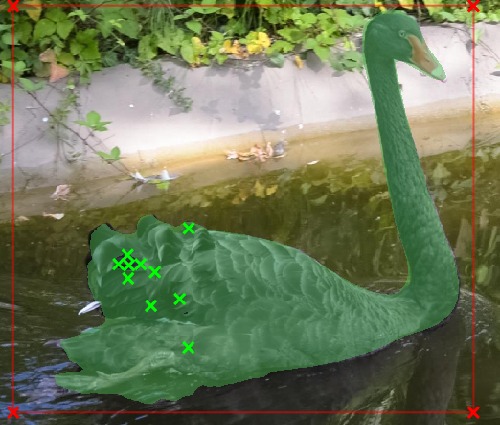
\includegraphics[width=\textwidth]{figures/appendix/method_predictions/swan34_iog.png}
		\caption{
			IOG $ IoU = 0.8805 $
		}
	\end{subfigure}
	\\
	% Pill defect
	\begin{subfigure}[t]{0.3\textwidth}
		\centering
		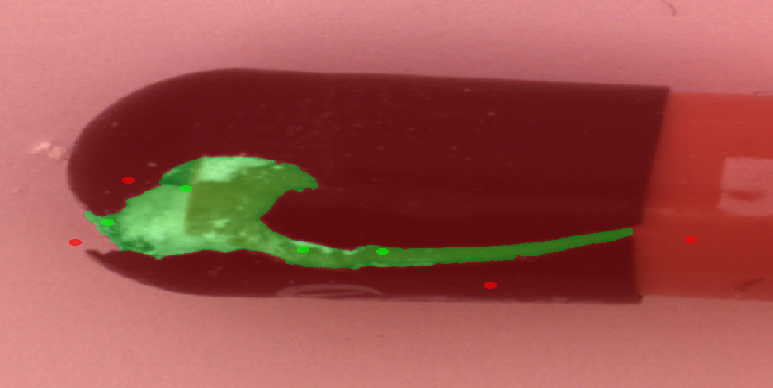
\includegraphics[width=\textwidth]{figures/appendix/method_predictions/pill78_watershed.png}
		\caption{
			Watershed $ IoU = 0.8173 $
		}
	\end{subfigure}
	\hfill
	\begin{subfigure}[t]{0.3\textwidth}
		\centering
		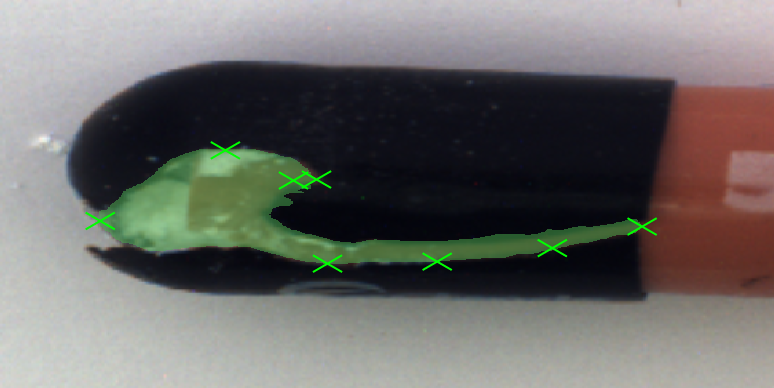
\includegraphics[width=\textwidth]{figures/appendix/method_predictions/pill78_dextr.png}
		\caption{
			DEXTR $ IoU = 0.8369 $
		}
	\end{subfigure}
	\hfill
	\begin{subfigure}[t]{0.3\textwidth}
		\centering
		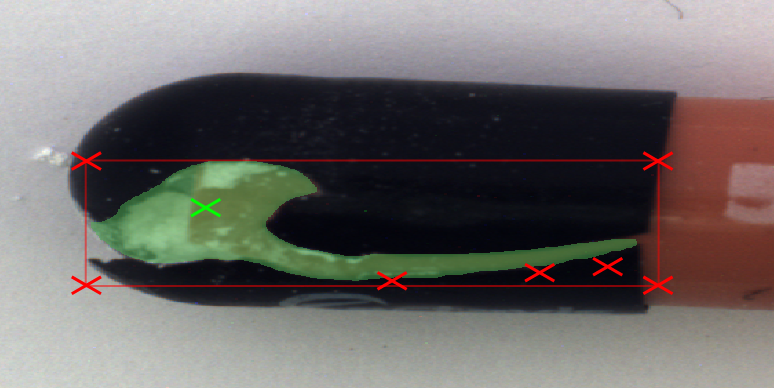
\includegraphics[width=\textwidth]{figures/appendix/method_predictions/pill78_iog.png}
		\caption{
			IOG $ IoU = 0.8605 $
		}
	\end{subfigure}
\end{figure}

%TODO also include some defects with low IoU